\documentclass{beamer}
\usepackage[utf8]{inputenc}
\usepackage{graphicx, epsfig}
\usepackage{amsmath,mathrsfs,amsfonts,amssymb}
\usepackage{floatflt}
\usepackage{epic,ecltree}
\usepackage{mathtext}
\usepackage{fancybox}
\usepackage{fancyhdr}
\usepackage{multirow}
\usepackage{enumerate}
\usepackage{epstopdf}
\usepackage{multicol}
\usepackage{algorithm}
\usepackage[noend]{algorithmic}
\usepackage{tikz}
\usepackage{blindtext}
\usetheme{default}%{Singapore}%{Warsaw}%{Warsaw}%{Darmstadt}
\usecolortheme{default}

\setbeamerfont{title}{size=\Huge}
\setbeamertemplate{footline}[page number]{}

\setbeamertemplate{section in toc}[sections numbered]


\makeatletter
\newcommand\HUGE{\@setfontsize\Huge{35}{40}}
\makeatother    

\setbeamerfont{title}{size=\HUGE}
\beamertemplatenavigationsymbolsempty

% latin bold lower
\newcommand{\ba}{\mathbf{a}} 
\newcommand{\bc}{\mathbf{c}} 
\newcommand{\be}{\mathbf{e}} 
\newcommand{\bh}{\mathbf{h}} 
\newcommand{\bp}{\mathbf{p}} 
\newcommand{\bt}{\mathbf{t}} 
\newcommand{\bs}{\mathbf{s}} 
\newcommand{\bu}{\mathbf{u}} 
\newcommand{\bv}{\mathbf{v}} 
\newcommand{\bw}{\mathbf{w}} 
\newcommand{\bx}{\mathbf{x}} 
\newcommand{\by}{\mathbf{y}} 
\newcommand{\bz}{\mathbf{z}} 

% latin bold upper
\newcommand{\bA}{\mathbf{A}} 
\newcommand{\bB}{\mathbf{B}} 
\newcommand{\bC}{\mathbf{C}} 
\newcommand{\bI}{\mathbf{I}} 
\newcommand{\bJ}{\mathbf{J}} 
\newcommand{\bL}{\mathbf{L}} 
\newcommand{\bM}{\mathbf{M}} 
\newcommand{\bQ}{\mathbf{Q}} 
\newcommand{\bT}{\mathbf{T}} 
\newcommand{\bU}{\mathbf{U}} 
\newcommand{\bV}{\mathbf{V}} 
\newcommand{\bW}{\mathbf{W}} 
\newcommand{\bX}{\mathbf{X}} 
\newcommand{\bY}{\mathbf{Y}} 
\newcommand{\bZ}{\mathbf{Z}} 

% latin cal upper
\newcommand{\cG}{\mathcal{G}} 
\newcommand{\cL}{\mathcal{L}} 
\newcommand{\cN}{\mathcal{N}} 
\newcommand{\cS}{\mathcal{S}} 
\newcommand{\cT}{\mathcal{T}} 
\newcommand{\cW}{\mathcal{W}} 
\newcommand{\cX}{\mathcal{X}} 
\newcommand{\cZ}{\mathcal{Z}} 

% latin bb upper
\newcommand{\bbE}{\mathbb{E}} 
\newcommand{\bbI}{\mathbb{I}} 
\newcommand{\bbP}{\mathbb{P}} 
\newcommand{\bbR}{\mathbb{R}} 

% greek bold lower
\newcommand{\bepsilon}{\boldsymbol{\epsilon}} 
\newcommand{\btheta}{\boldsymbol{\theta}} 
\newcommand{\blambda}{\boldsymbol{\lambda}} 
\newcommand{\bpi}{\boldsymbol{\pi}} 
\newcommand{\bmu}{\boldsymbol{\mu}} 
\newcommand{\bsigma}{\boldsymbol{\sigma}} 
\newcommand{\bphi}{\boldsymbol{\phi}} 

% greek bold upper
\newcommand{\bSigma}{\boldsymbol{\Sigma}} 

\DeclareMathOperator*{\argmin}{arg\,min}
\DeclareMathOperator*{\argmax}{arg\,max}

\newcommand{\createdgmtitle}[1]{\title[\hbox to 56mm{Deep Learning Audio \hfill\insertframenumber\,/\,\inserttotalframenumber}]
	{\vspace{1cm} \\ Deep Learning Audio \\ {\Huge Lecture #1}}
	\author{Pavel Severilov}
	\institute{
	Moscow Institute of Physics and Technology
	} 
	\date{2022}
}

\newcommand\myfootnote[1]{%
  \tikz[remember picture,overlay]
  \draw (current page.south west) +(1in + \oddsidemargin,0.5em)
  node[anchor=south west,inner sep=0pt]{\parbox{\textwidth}{%
      \rlap{\rule{10em}{0.4pt}}\raggedright\scriptsize \textit{#1}}};}

\newcommand\myfootnotewithlink[2]{%
  \tikz[remember picture,overlay]
  \draw (current page.south west) +(1in + \oddsidemargin,0.5em)
  node[anchor=south west,inner sep=0pt]{\parbox{\textwidth}{%
      \rlap{\rule{10em}{0.4pt}}\raggedright\scriptsize\href{#1}{\textit{#2}}}};}
      
\AtBeginSection[]
{
	\begin{frame}{Outline}
		\tableofcontents[currentsection,subsectionstyle=hide]
	\end{frame}
}
\AtBeginSubsection[]{
	\begin{frame}{Outline}
		\tableofcontents[currentsection,currentsubsection]
	\end{frame}
}
\createdgmtitle{2}
\usepackage{tikz}
\usetikzlibrary{arrows,shapes,positioning,shadows,trees}
%--------------------------------------------------------------------------------
\begin{document}
%--------------------------------------------------------------------------------
\begin{frame}[noframenumbering,plain]
%\thispagestyle{empty}
\titlepage
\end{frame}
%=======x
\begin{frame}{Outline}
	\tableofcontents
\end{frame}
%=======
\section{Sound: Introduction}
%=======
\begin{frame}{Mind experiment: what is sound?}
		\begin{figure}
			\centering
			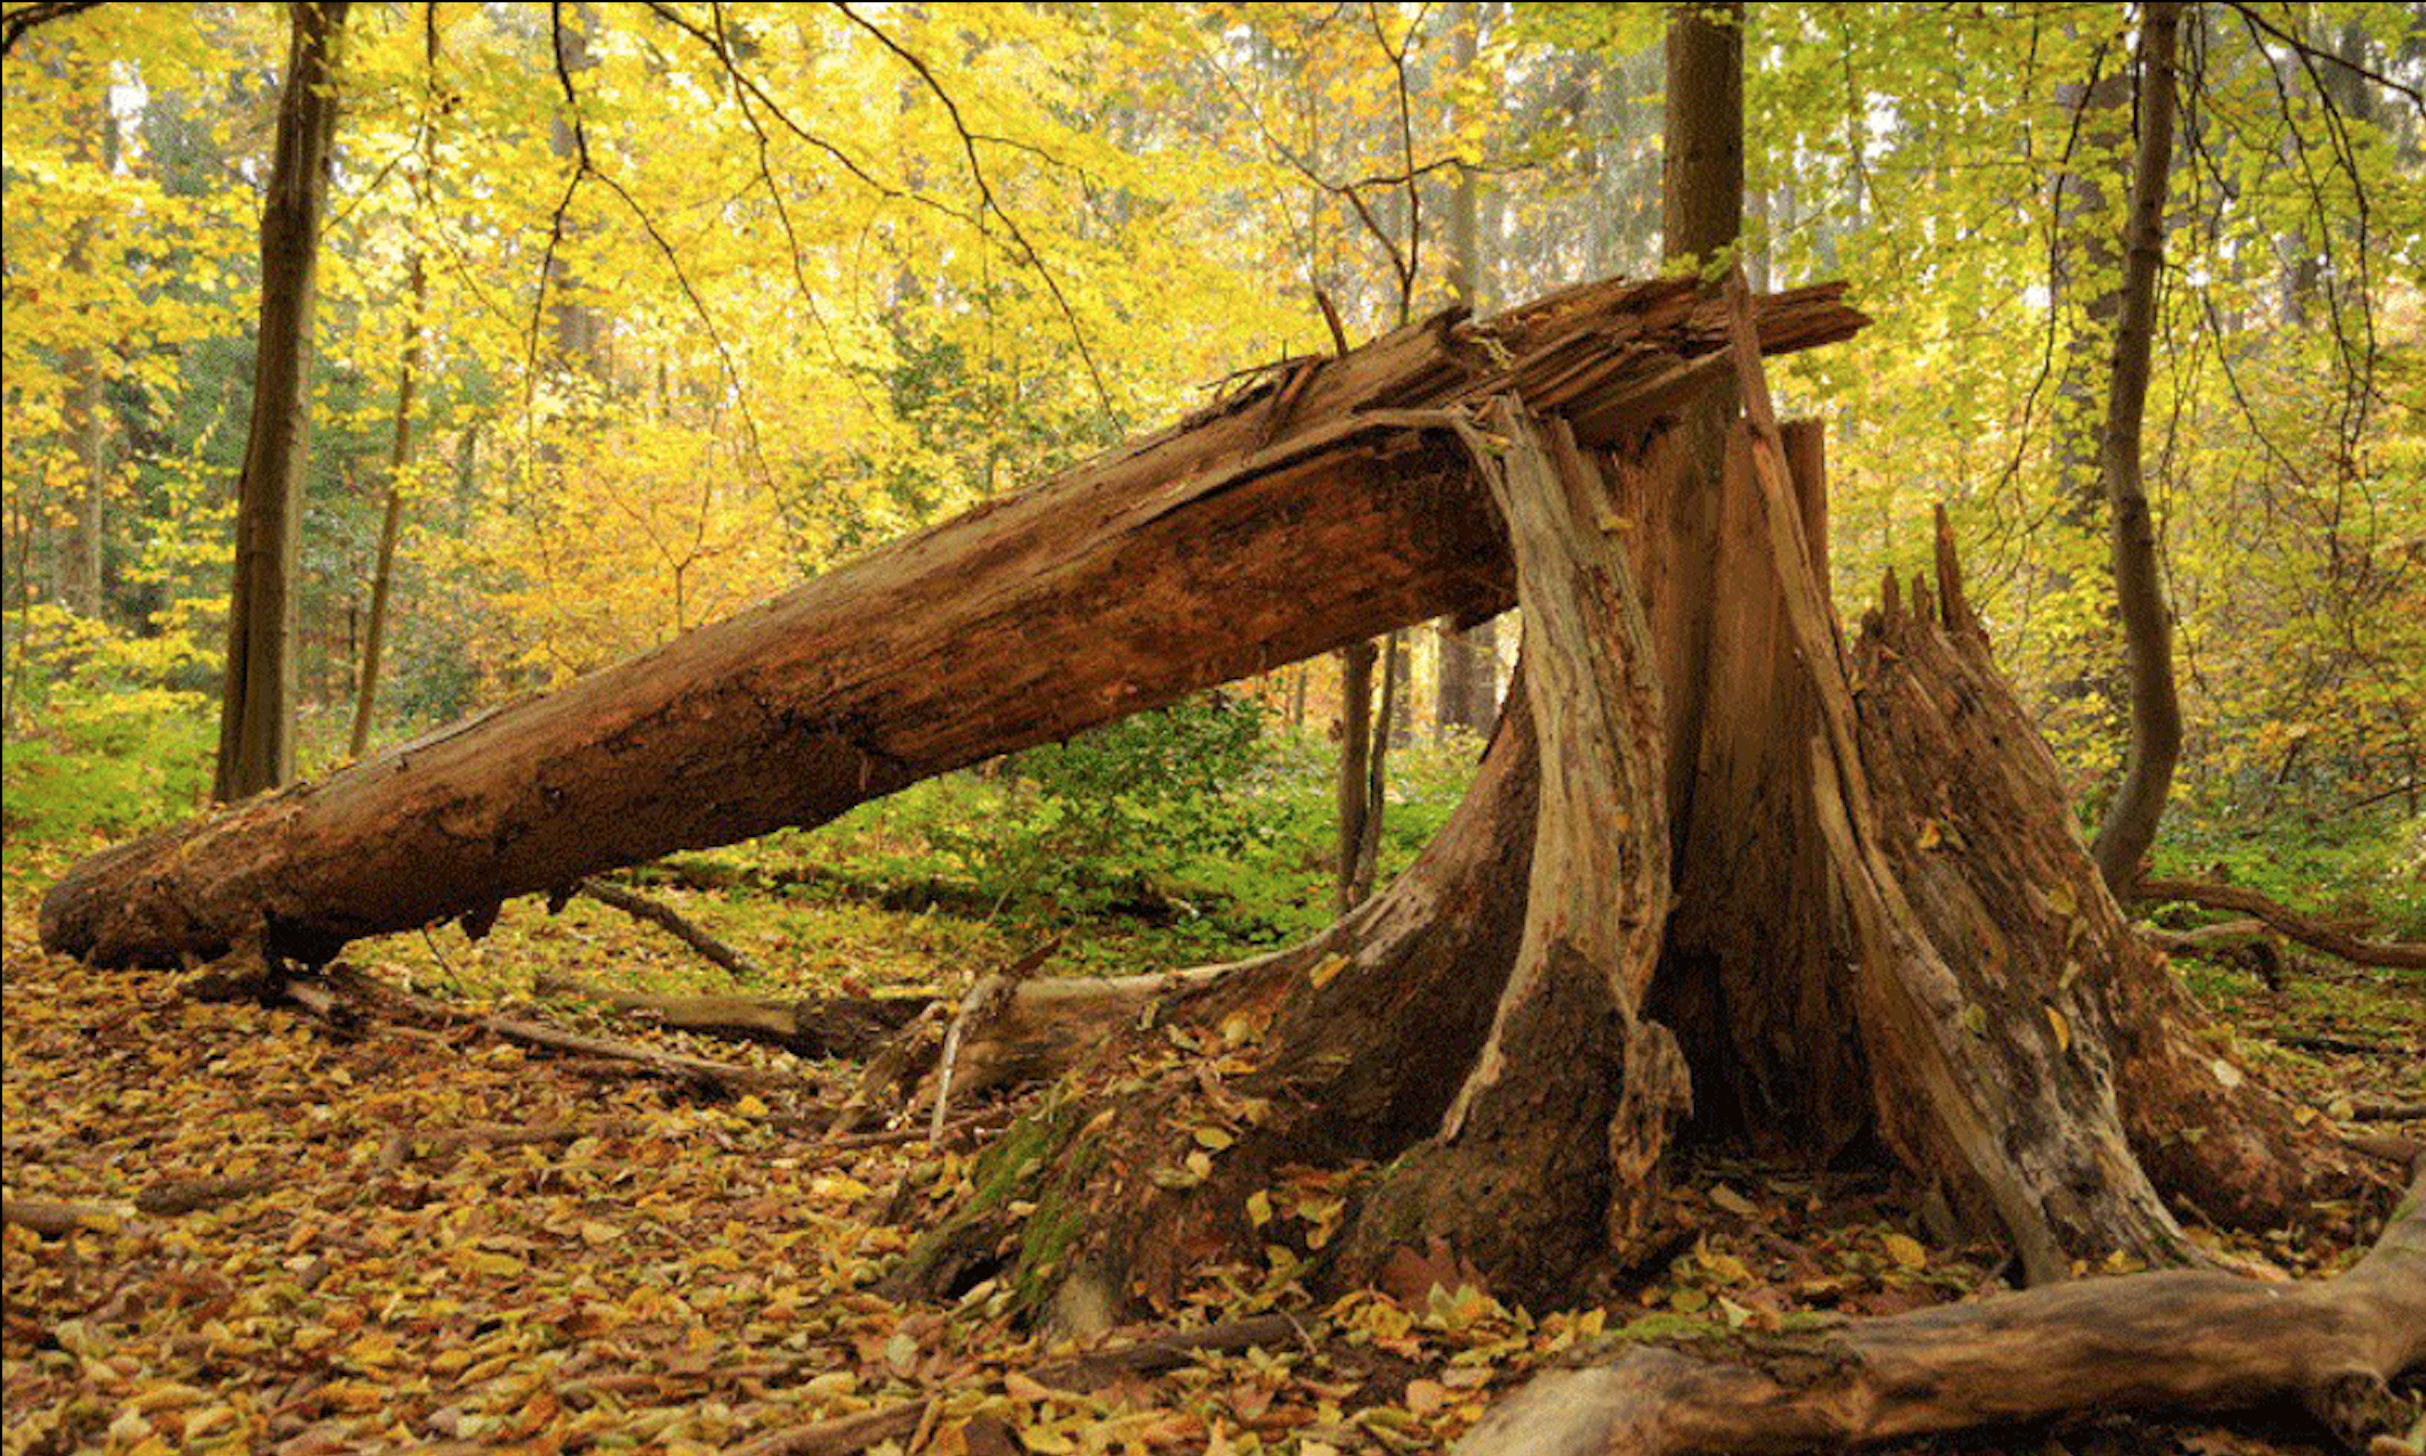
\includegraphics[width=0.99\linewidth]{figs/tree_forest.png}
			\caption{If a tree falls in the forest, and there’s nobody around to hear, does it make a sound?}
		\end{figure}
\end{frame}
%=======
\begin{frame}{Ear structure}
	\begin{figure}
		\centering
		\includegraphics[width=0.99\linewidth]{figs/ear_structure.png}
		\caption{Fourier decomposition in our body}
	\end{figure}
	Fourier transform of a signal $x(t)$
	$$
	\mathcal{F}\{x(t)\}=X(j \omega)=\int_{-\infty}^{\infty} x(t) e^{-j \omega t} d t
	$$
\end{frame}
%=======
\section{Sound: characteristics}
%=======
\begin{frame}{Sound types: analog vs digital}
		\begin{itemize}
			\item For any $T > 0$, we may sample a \textbf{Continuous-Time} (CT) signal $x(t)$ to generate the \textbf{Discrete-Time} (DT) signal $x[n]=x(nT)$
			\item DT: signal $x(t)$ is evaluating at uniformly spaced points on the t-axis. The number T is the \textbf{sampling period}
			\item \textbf{Sampling frequency}: $f_s=\frac{1}{T}$, {[Hertz or samples/sec.]}
		\end{itemize}
	\begin{figure}
		\centering
		\includegraphics[width=0.6\linewidth]{figs/analog_discrete.png}
	\end{figure}
\end{frame}
%=======
\begin{frame}{Sound characteristics}
	\begin{itemize}
		\item Signal $x(t)$
		\item Signal energy $\int_{-\infty}^{\infty}|x(t)|^2 d t$ (used for normalizing signals, augmentations)
		\item Sample rate (SR) -- number of audio samples per one second
			\begin{itemize}
				\item 8 kHz or 16 kHz - standart for audio in telephony
				\item 44.1 kHz - CD audio/Computer Audio
				\item 48 kHz - DVD audio/Computer Audio
				\item 96 kHz - High resolution Audio
			\end{itemize}
		\item Number of channels -- how many signals we record in parallel (mono: 1, stereo: 2)
	\end{itemize}
\end{frame}
%=======
\begin{frame}{The Nyquist Theorem}
	\begin{itemize}
		\item $\Sigma_{C T}$ -- set of all CT signals $x(t)$, $\Sigma_{D T}$ -- set of all DT signals $x[n]$. Procedure of sampling for a given sampling period $T$:
		$$
		\Sigma_{C T} \longmapsto \Sigma_{D T} ~~\Leftrightarrow ~~x(t) \longmapsto x[n]=x(n T)
		$$
		\item CT signal $x(t)$ is bandlimited if there exists $\omega_B<\infty$ such that $X_{C T}(j \omega)=0$ for $|\omega|>\omega_B$
	\end{itemize}
	
	\begin{block}{Nyquist Theorem}
		The sampling map is bijection on $\Sigma_{\omega_B}$ iff $\omega_s>2 \omega_B$. $\omega_s=2 \pi f_s=\frac{2 \pi}{T}$ -- radian sampling frequency
	\end{block}
\begin{figure}
	\centering
	\includegraphics[width=0.38\linewidth]{figs/nyquist.png}
\end{figure}
\end{frame}
%=======

\section{Fourier Transform}
%=======
\begin{frame}{Fourier Transform: motivation}
	\begin{figure}
		\centering
		\includegraphics[width=0.8\linewidth]{figs/signal_decomposition.png}
		\caption{Fourier Transform transfer a signal from the \textbf{time domain} to the \textbf{frequency domain}}
	\end{figure}
\end{frame}
%=======
%=======
\begin{frame}{Fourier Transform}
	\begin{itemize}
		\item CT Fourier transform (CTFT) of a CT signal $x(t)$ is $$\mathcal{F}\{x(t)\}=X(j \omega)=\int_{-\infty}^{\infty} x(t) e^{-j \omega t} d t$$
		\item CT unit impulse $\delta(t)$, $\int_{-\infty}^{\infty} \delta(t) d t=1,$
		\item Define signal by CT impulse $x(t)=\sum_{n=-\infty}^{\infty} x[n] \delta(t-n)$
		\item 	Taking Fourier transform for DT signal: 
		$$
		\begin{aligned}
		X(j \omega) &=\int_{-\infty}^{\infty} \sum_{n=-\infty}^{\infty} x[n] \delta(t-n) e^{-j \omega t} d t \\
		&=\sum_{n=-\infty}^{\infty} x[n] e^{-j \omega n} \int_{-\infty}^{\infty} \delta(t-n) e^{-j \omega (t-n)}d t \\
		&=\sum_{n=-\infty}^{\infty} x[n] e^{-j \omega n} = \mathbf{M} x(t).
		\end{aligned}$$
	\end{itemize}
\end{frame}

%=======
\begin{frame}{DTFT: example}
\begin{figure}
	\centering
	\includegraphics[width=0.8\linewidth]{figs/signal_spectrum.png}
	\caption{Example of DTFT for cosine signal}
\end{figure}
\end{frame}
%=======
\begin{frame}{Problems with Fourier Transorm in real life}
	\begin{figure}
		\centering
		\includegraphics[width=0.99\linewidth]{figs/fourier_problems.png}
	\end{figure}
\myfootnotewithlink{https://github.com/yandexdataschool/speech\_course}{HSE DLA course}
\end{frame}

%=======
\begin{frame}{Short-time Fourier Transform (STFT)}
\begin{figure}
	\centering
	\includegraphics[width=0.99\linewidth]{figs/stft.png}
\end{figure}
STFT (DTFT with Hamming window): $$X[r, w)=\sum_{n=-\infty}^{\infty} w[r-n] x[n] e^{-j \omega n},$$ where $w$ -- window function, $r$ -- location of window along the time axis
\end{frame}
%=======
\section{Spectrograms}
%=======
\begin{frame}{Spectrograms}
	\begin{figure}
		\centering
		\includegraphics[width=0.8\linewidth]{figs/stft_spec.png}
		\caption{STFT+window Spectrogram }
	\end{figure}
\end{frame}
%=======
\begin{frame}{Mel Scale}
	\begin{itemize}
		\item Mel Scale: humans percieve sound on a log-scale, not linear
		\item A lot of formulas to convert f hertz into m mels. Popular example: $$m=2595 \log _{10}\left(1+\frac{f}{700}\right)$$
	\end{itemize} 
	\begin{figure}
	\centering
	\includegraphics[width=0.8\linewidth]{figs/mel_scale.png}
	\caption{Mel scale}
\end{figure}
\end{frame}
%=======
\begin{frame}{Mel spectrogram}
	\begin{figure}
		\centering
		\includegraphics[width=0.8\linewidth]{figs/mel_spectrogram.png}
		\caption{Waveform $\rightarrow$ STFT+window Spectrogram $\rightarrow$ STFT+window+Mel scale Spectrogram}
	\end{figure}
\end{frame}

\end{document} 